\documentclass[tikz,border=2pt]{standalone}
\usepackage{amsmath,amssymb}
\usepackage{pgfplots}
\pgfplotsset{compat=1.18}

\begin{document}
% Conditioning on B = {X >= 3} keeps only the values in B and rescales their probabilities
% by P(B) = 0.7; the conditional expectation is the mean of this new pmf: E[X | B] = 25/7.
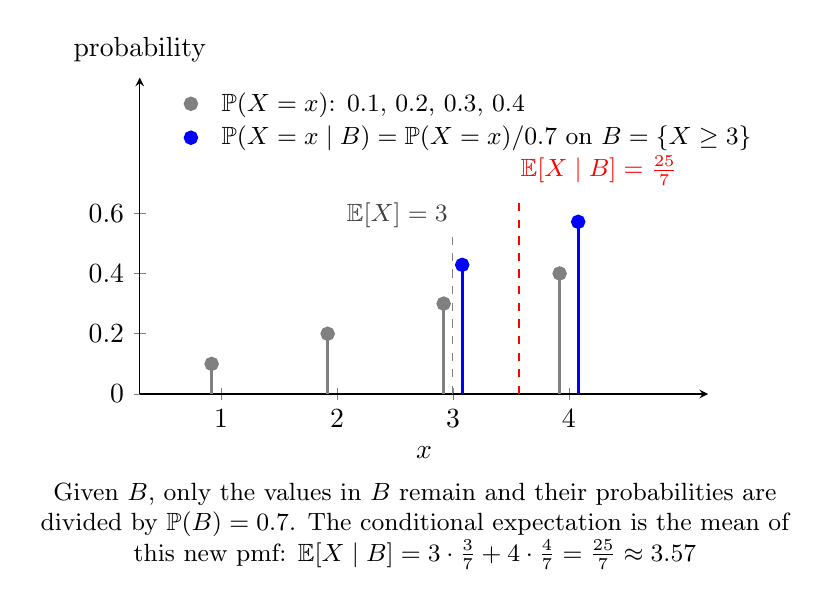
\begin{tikzpicture}
	\begin{axis}[
		axis lines=left, xmin=0.3, xmax=5.2, ymin=0, ymax=1.05,
		xtick={1,2,3,4}, ytick={0,0.2,0.4,0.6},
		xlabel={$x$}, ylabel={probability}, ylabel style={rotate=-90, anchor=south, at={(axis description cs:0,1.02)}},
		width=8.8cm, height=5.6cm, clip=false,
		legend style={draw=none, fill=none, font=\small, at={(0.03,0.99)}, anchor=north west}, legend cell align=left
		]
		\addplot[ycomb, gray, very thick, mark=*, mark size=2pt] coordinates {(0.92,0.1) (1.92,0.2) (2.92,0.3) (3.92,0.4)};
		\addlegendentry{$\mathbb{P}(X=x)$: $0.1,\,0.2,\,0.3,\,0.4$}
		\addplot[ycomb, blue, very thick, mark=*, mark size=2pt] coordinates {(3.08,0.4286) (4.08,0.5714)};
		\addlegendentry{$\mathbb{P}(X=x\mid B)=\mathbb{P}(X=x)/0.7$ on $B=\{X\ge3\}$}
		\draw[red, dashed, thick] (axis cs:3.571,0) -- (axis cs:3.571,0.66);
		\node[red, anchor=south west, font=\small] at (axis cs:3.5,0.66) {$\mathbb{E}[X\mid B]=\tfrac{25}7$};
		\draw[gray, dashed] (axis cs:3,0) -- (axis cs:3,0.52);
		\node[gray!50!black, anchor=south east, font=\small] at (axis cs:3.04,0.52) {$\mathbb{E}[X]=3$};
	\end{axis}
	\node[anchor=north, font=\small, align=flush center, text width=9.6cm] at ([yshift=-2pt]current axis.outer south) {Given $B$, only the values in $B$ remain and their probabilities are divided by $\mathbb{P}(B)=0.7$. The conditional expectation is the mean of this new pmf: $\mathbb{E}[X\mid B]=3\cdot\tfrac37+4\cdot\tfrac47=\tfrac{25}7\approx3.57$};
\end{tikzpicture}
\end{document}
